\section{Time series analysis}

\subsection{Overview}
In this section we will analyse the dataset \textit{CityGlobalTemperature2000-2009.csv} a collection of temperature measurements from 100 cities. For each record we had
\begin{itemize}
    \item \textbf{AverageTemperature}: the measurament of the average temperature.
    \item \textbf{AverageTemperatureUncertainty}: the measurament of the temperature standard deviation.
    \item \textbf{City}: the city related to the measurement.
    \item \textbf{Country}, \textbf{Longitude}, \textbf{Latitude}: of the related city.
    \item \textbf{Time}: with respect to when the measurement was made.
\end{itemize}
with data spanning across 10 years.
We will exploit this data to find a meaningful group of cities with respect to temperature trends.
\subsection{Data Analysis}
We initially plotted \textit{AverageTemperature} and \textit{AverageTemperatureUncertainty} attributes regarding some random cities with respect to the time in which they were measured to find some patterns.\\
While for \textit{AverageTemperature} we can observe the cyclic behaviour derived from the seasonality \ref{fig:average_temperature} for what it regards \textit{AverageTemperatureUncertainty} we couldn't find a pattern via this view \ref{fig:average_temperature_uncertainty}.
\begin{figure}[h]
	\centering
	\begin{minipage}{.48\textwidth}
    	\centering
    	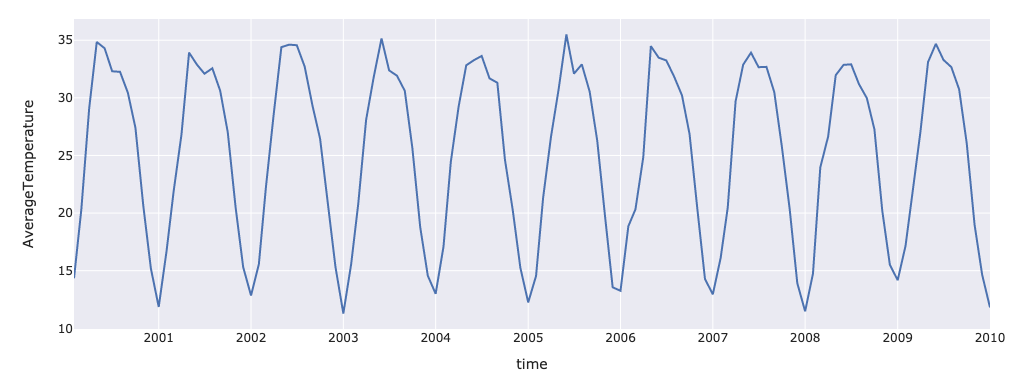
\includegraphics[width=\textwidth]{plots/timeseries/Average Temperature.png}
    	\subcaption{Average Temperature of Lahore city}
    	\label{fig:average_temperature}
	\end{minipage}%
    \begin{minipage}{.48\textwidth}
    	\centering
    	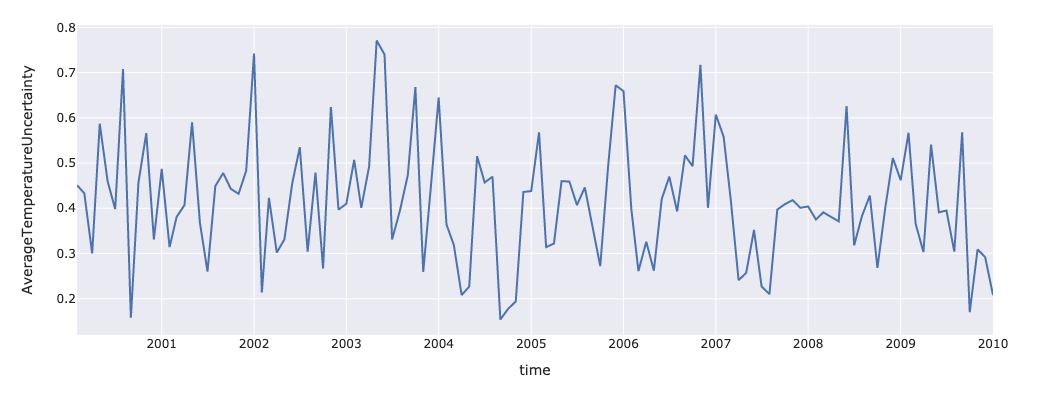
\includegraphics[width=\textwidth]{plots/timeseries/Average Temperature Uncertainty.png}
    	\subcaption{Average Temperature Uncertainty of Rome city}
    	\label{fig:average_temperature_uncertainty}
    \end{minipage}
    \captionof{figure}{Average temperatures plot.}
\end{figure}\\
\subsection{Data Transformation \& Feature Engineering}
In this phase we created a new dataset (\textit{df\_city}) where each record was related to a particular city, and we added features composed ad hoc for the clustering.\\
We decided to create:
\begin{itemize}
    \item $12$ feature \textit{\textbf{month\_avg}} where each one represent the average temperature in a given month (\textit{AverageTemperature}) averaged over all the years with respect to a given city.
    \item $12$ feature \textit{\textbf{month\_var}} where each one represent the temperature variance in a given month (\textit{AverageTemperatureUncertainty}) averaged over all the years  with respect to a given city.
    \item One last feature, \textit{\textbf{AverageTemperatureUncertainty}} regarding temperature variance of a given city averaged over all the months and all the years. this feature was created if the previous one did not lead to good results and if the variance of the average temperature was not a parameter dependent on the month in which it is measured.
\end{itemize} 
\subsection{Clustering}
In these phases, we apply the k-means clustering algorithm using different metrics to compute the distance and different combinations of features.\\
We tried the following combinations of features with euclidean distance as a metric:
\begin{enumerate}
    \item Just the $12$ \textit{month\_avg} features.
    \item Just the $12$ \textit{month\_var} features.
    \item The $12$ \textit{month\_avg} features combined with the other $12$ \textit{month\_var} features.
    \item The $12$ \textit{month\_avg} features combined with the other $12$ \textit{month\_var} features.
    \item The $12$ \textit{month\_avg} features combined with the \textit{AverageTemperatureUncertainty} feature.
\end{enumerate}
The best results were obtained with the first configuration, where we set k=7 as the number of cluster.\\
\begin{figure}[h]
	\centering
	\begin{minipage}{.33\textwidth}
		\centering
		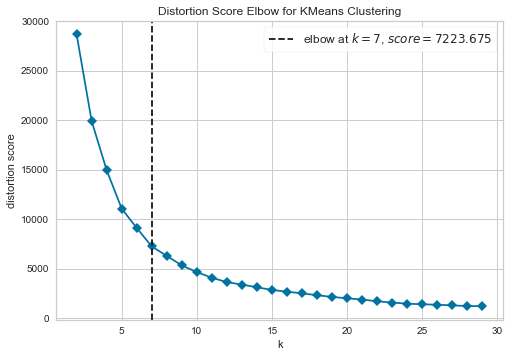
\includegraphics[width=\textwidth]{plots/timeseries/distortion_score.png}
		\subcaption{Distortion Score}
		\label{fig:distortion_score}
	\end{minipage}%
	\begin{minipage}{.33\textwidth}
		\centering
		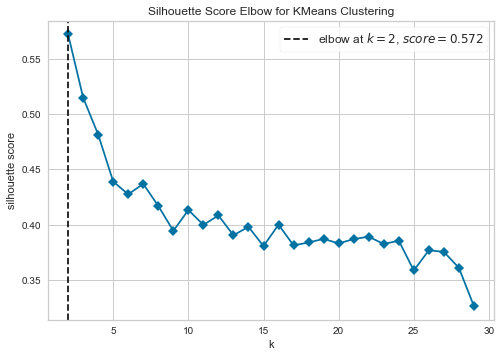
\includegraphics[width=\textwidth]{plots/timeseries/silhouette score.png}
		\subcaption{Silhouette score}
		\label{fig:silhouette_score}
	\end{minipage}
	\begin{minipage}{.33\textwidth}
	    \centering
	    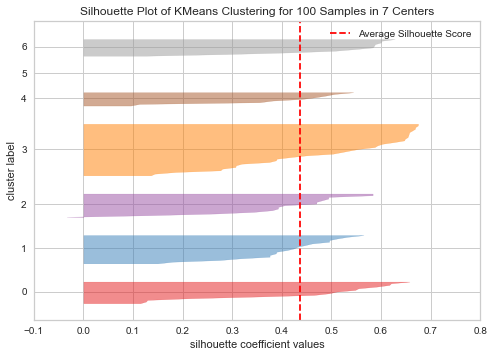
\includegraphics[width=\textwidth]{plots/timeseries/silhouette score 2.png}
	    \subcaption{Cluster Silhouette score}
	    \label{fig:silhouette_score2}
	\end{minipage}
\end{figure}\\
We obtained a silhouette score of 0.4369 but what it was more appreciable was the semantic meaning.
We can observe how each cluster described a different seasonality \ref{fig:centroids} and how group of cities are in correspondence with a given a latitude which typically characterized cold or hot places \ref{fig:geoplot}.\\
\begin{figure}[h!]
		\centering
		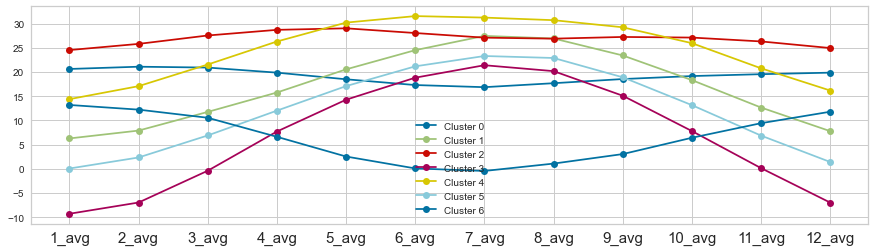
\includegraphics[width=0.8\textwidth]{plots/timeseries/centroids.png}
		\subcaption{Clustering centroids}
		\label{fig:centroids}
\end{figure}
\begin{figure}[h!]
		\centering
		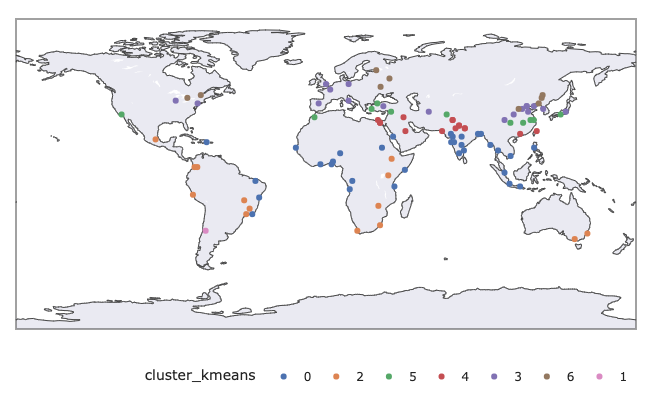
\includegraphics[width=0.8\textwidth]{plots/timeseries/geoplot.png}
		\subcaption{Plot on the world map}
		\label{fig:geoplot}
\end{figure}
\subsubsection{Further experiments}
Trying to cluster on the variance features of the temperature results in worst results with respect to the average. So in case those results were caused by a misalignment in the time series, we tried to approach the clustering by exploiting a Dynamic Time Warping distance in combination with k-means instead of the euclidean distance.\\
However, even with this attempt, the results tend to be almost equal to the Euclidean distance:

\begin{figure}[h!]
	\centering
	\begin{minipage}{.5\textwidth}
		\centering
		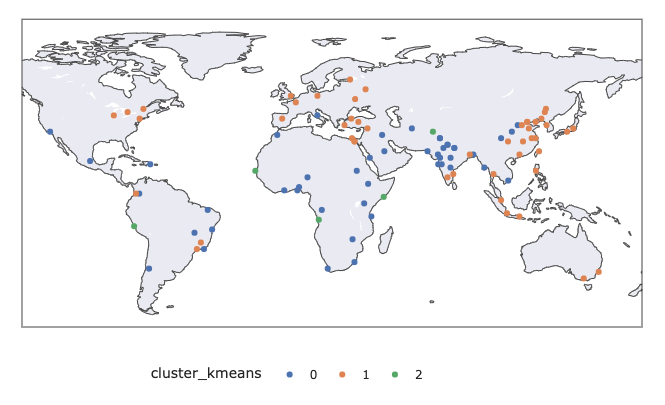
\includegraphics[width=\textwidth]{plots/timeseries/geoplot_var.png}
		\subcaption{World map plot with euclidean distance}
		\label{fig:geoplot_var}
	\end{minipage}%
	\begin{minipage}{.5\textwidth}
		\centering
		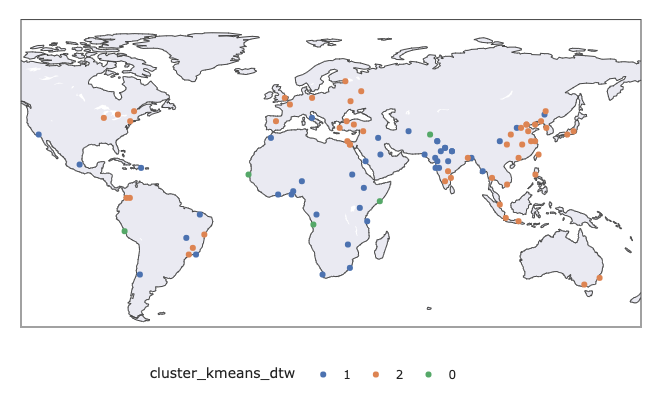
\includegraphics[width=\textwidth]{plots/timeseries/geoplot_var_dtw.png}
		\subcaption{World map plot with Dynamic Time Warping distance}
		\label{fig:geoplot_var_dtw}
	\end{minipage}
\end{figure}\\